\documentclass[tikz,border=10pt]{standalone}
\usepackage{tikz}
\usetikzlibrary{arrows.meta,positioning,calc}

% Define KUL colors to match your style
\definecolor{KUL-BLUE}{RGB}{29, 55, 104}
\definecolor{KUL-RED}{RGB}{170, 30, 30}
\definecolor{KUL-ORANGE}{RGB}{230, 140, 0}
\definecolor{KUL-GREEN}{RGB}{0, 128, 0}

\begin{document}

% Frame 0: Initial setup with both sets
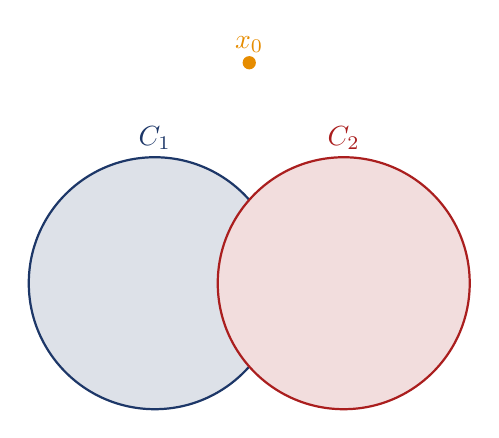
\begin{tikzpicture}[scale=0.8]
  % Set C1 (left circle)
  \fill[KUL-BLUE!15, draw=KUL-BLUE, thick] (-1.5,-0.5) circle (2.0);
  \node[KUL-BLUE] at (-1.5,1.8) {$C_1$};
  
  % Set C2 (right circle)
  \fill[KUL-RED!15, draw=KUL-RED, thick] (1.5,-0.5) circle (2.0);
  \node[KUL-RED] at (1.5,1.8) {$C_2$};
  
  % Starting point
  \fill[KUL-ORANGE] (0,3.0) circle (3pt);
  \node[KUL-ORANGE, above] at (0,3.0) {$x_0$};
\end{tikzpicture}

% Frame 1: First projection to C1
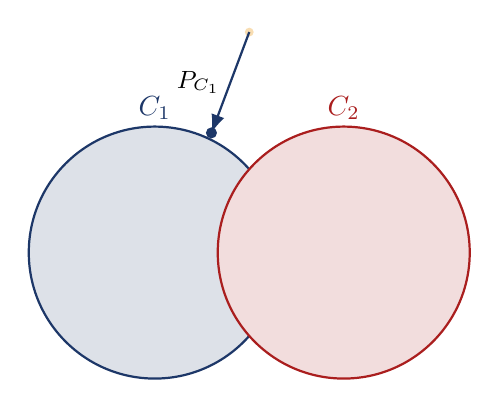
\begin{tikzpicture}[scale=0.8]
  % Set C1 (left circle)
  \fill[KUL-BLUE!15, draw=KUL-BLUE, thick] (-1.5,-0.5) circle (2.0);
  \node[KUL-BLUE] at (-1.5,1.8) {$C_1$};
  
  % Set C2 (right circle)
  \fill[KUL-RED!15, draw=KUL-RED, thick] (1.5,-0.5) circle (2.0);
  \node[KUL-RED] at (1.5,1.8) {$C_2$};
  
  % Starting point
  \fill[KUL-ORANGE!30] (0,3.0) circle (2pt);
  
  % Projection to C1
  \coordinate (start) at (0,3.0);
  \coordinate (p1) at (-0.6,1.4);
  
  \draw[->, >=Latex, KUL-BLUE, thick] (start) -- (p1)
    node[midway, left, font=\small, black] {$P_{C_1}$};
  \fill[KUL-BLUE] (p1) circle (2.5pt);
\end{tikzpicture}

% Frame 2: First projection to C2
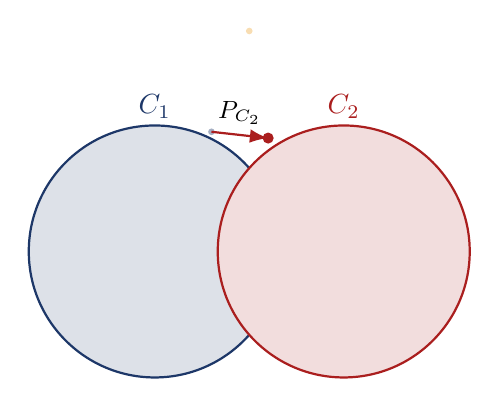
\begin{tikzpicture}[scale=0.8]
  % Set C1 (left circle)
  \fill[KUL-BLUE!15, draw=KUL-BLUE, thick] (-1.5,-0.5) circle (2.0);
  \node[KUL-BLUE] at (-1.5,1.8) {$C_1$};
  
  % Set C2 (right circle)
  \fill[KUL-RED!15, draw=KUL-RED, thick] (1.5,-0.5) circle (2.0);
  \node[KUL-RED] at (1.5,1.8) {$C_2$};
  
  % Previous points (faded)
  \fill[KUL-ORANGE!30] (0,3.0) circle (1.5pt);
  \fill[KUL-BLUE!40] (-0.6,1.4) circle (1.5pt);
  
  % Projection to C2
  \coordinate (p1) at (-0.6,1.4);
  \coordinate (p2) at (0.3,1.3);
  
  \draw[->, >=Latex, KUL-RED, thick] (p1) -- (p2)
    node[midway, above, font=\small, black] {$P_{C_2}$};
  \fill[KUL-RED] (p2) circle (2.5pt);
\end{tikzpicture}

% Frame 3: Second iteration - projection to C1
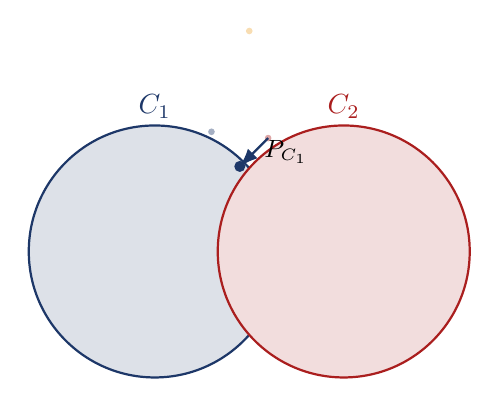
\begin{tikzpicture}[scale=0.8]
  % Set C1 (left circle)
  \fill[KUL-BLUE!15, draw=KUL-BLUE, thick] (-1.5,-0.5) circle (2.0);
  \node[KUL-BLUE] at (-1.5,1.8) {$C_1$};
  
  % Set C2 (right circle)
  \fill[KUL-RED!15, draw=KUL-RED, thick] (1.5,-0.5) circle (2.0);
  \node[KUL-RED] at (1.5,1.8) {$C_2$};
  
  % Previous points (faded)
  \fill[KUL-ORANGE!30] (0,3.0) circle (1.5pt);
  \fill[KUL-BLUE!40] (-0.6,1.4) circle (1.5pt);
  \fill[KUL-RED!40] (0.3,1.3) circle (1.5pt);
  
  % Projection to C1
  \coordinate (p2) at (0.3,1.3);
  \coordinate (p3) at (-0.15,0.85);
  
  \draw[->, >=Latex, KUL-BLUE, thick] (p2) -- (p3)
    node[midway, right, font=\small, black] {$P_{C_1}$};
  \fill[KUL-BLUE] (p3) circle (2.5pt);
\end{tikzpicture}

% Frame 4: Second iteration - projection to C2
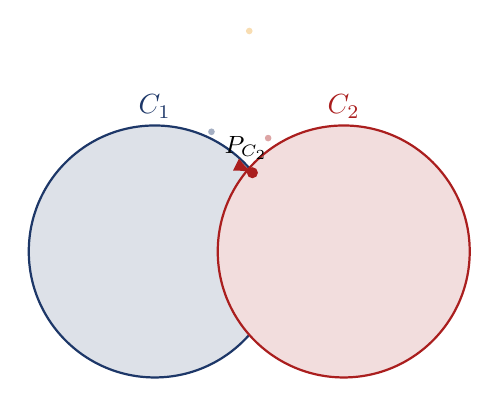
\begin{tikzpicture}[scale=0.8]
  % Set C1 (left circle)
  \fill[KUL-BLUE!15, draw=KUL-BLUE, thick] (-1.5,-0.5) circle (2.0);
  \node[KUL-BLUE] at (-1.5,1.8) {$C_1$};
  
  % Set C2 (right circle)
  \fill[KUL-RED!15, draw=KUL-RED, thick] (1.5,-0.5) circle (2.0);
  \node[KUL-RED] at (1.5,1.8) {$C_2$};
  
  % Previous points (faded)
  \fill[KUL-ORANGE!30] (0,3.0) circle (1.5pt);
  \fill[KUL-BLUE!40] (-0.6,1.4) circle (1.5pt);
  \fill[KUL-RED!40] (0.3,1.3) circle (1.5pt);
  \fill[KUL-BLUE!40] (-0.15,0.85) circle (1.5pt);
  
  % Projection to C2
  \coordinate (p3) at (-0.15,0.85);
  \coordinate (p4) at (0.05,0.75);
  
  \draw[->, >=Latex, KUL-RED, thick] (p3) -- (p4)
    node[midway, above, font=\small, black] {$P_{C_2}$};
  \fill[KUL-RED] (p4) circle (2.5pt);
\end{tikzpicture}

% Frame 5: Third iteration - projection to C1
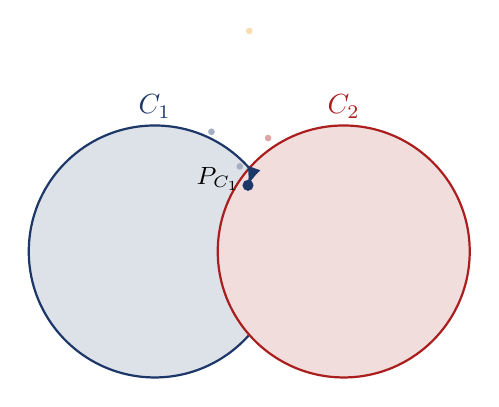
\begin{tikzpicture}[scale=0.8]
  % Set C1 (left circle)
  \fill[KUL-BLUE!15, draw=KUL-BLUE, thick] (-1.5,-0.5) circle (2.0);
  \node[KUL-BLUE] at (-1.5,1.8) {$C_1$};
  
  % Set C2 (right circle)
  \fill[KUL-RED!15, draw=KUL-RED, thick] (1.5,-0.5) circle (2.0);
  \node[KUL-RED] at (1.5,1.8) {$C_2$};
  
  % Previous points (faded)
  \fill[KUL-ORANGE!30] (0,3.0) circle (1.5pt);
  \fill[KUL-BLUE!40] (-0.6,1.4) circle (1.5pt);
  \fill[KUL-RED!40] (0.3,1.3) circle (1.5pt);
  \fill[KUL-BLUE!40] (-0.15,0.85) circle (1.5pt);
  \fill[KUL-RED!40] (0.05,0.75) circle (1.5pt);
  
  % Projection to C1
  \coordinate (p4) at (0.05,0.75);
  \coordinate (p5) at (-0.02,0.55);
  
  \draw[->, >=Latex, KUL-BLUE, thick] (p4) -- (p5)
    node[midway, left, font=\small, black] {$P_{C_1}$};
  \fill[KUL-BLUE] (p5) circle (2.5pt);
\end{tikzpicture}

% Frame 6: Third iteration - projection to C2
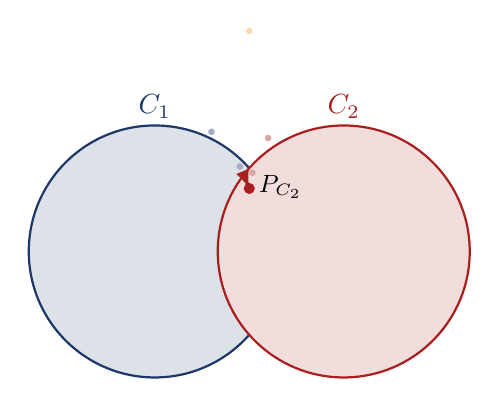
\begin{tikzpicture}[scale=0.8]
  % Set C1 (left circle)
  \fill[KUL-BLUE!15, draw=KUL-BLUE, thick] (-1.5,-0.5) circle (2.0);
  \node[KUL-BLUE] at (-1.5,1.8) {$C_1$};
  
  % Set C2 (right circle)
  \fill[KUL-RED!15, draw=KUL-RED, thick] (1.5,-0.5) circle (2.0);
  \node[KUL-RED] at (1.5,1.8) {$C_2$};
  
  % Previous points (faded)
  \fill[KUL-ORANGE!30] (0,3.0) circle (1.5pt);
  \fill[KUL-BLUE!40] (-0.6,1.4) circle (1.5pt);
  \fill[KUL-RED!40] (0.3,1.3) circle (1.5pt);
  \fill[KUL-BLUE!40] (-0.15,0.85) circle (1.5pt);
  \fill[KUL-RED!40] (0.05,0.75) circle (1.5pt);
  \fill[KUL-BLUE!40] (-0.02,0.55) circle (1.5pt);
  
  % Projection to C2
  \coordinate (p5) at (-0.02,0.55);
  \coordinate (p6) at (0.0,0.5);
  
  \draw[->, >=Latex, KUL-RED, thick] (p5) -- (p6)
    node[midway, right, font=\small, black] {$P_{C_2}$};
  \fill[KUL-RED] (p6) circle (2.5pt);
\end{tikzpicture}

% Frame 7: Final convergence with intersection
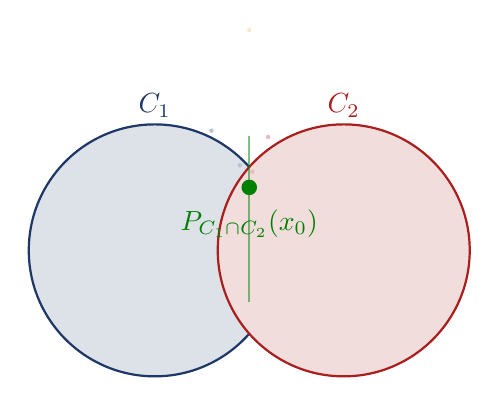
\begin{tikzpicture}[scale=0.8]
  % Set C1 (left circle)
  \fill[KUL-BLUE!15, draw=KUL-BLUE, thick] (-1.5,-0.5) circle (2.0);
  \node[KUL-BLUE] at (-1.5,1.8) {$C_1$};
  
  % Set C2 (right circle)
  \fill[KUL-RED!15, draw=KUL-RED, thick] (1.5,-0.5) circle (2.0);
  \node[KUL-RED] at (1.5,1.8) {$C_2$};
  
  % Intersection line
  \draw[KUL-GREEN, thick, opacity=0.5] (0,-1.32) -- (0,1.32);
  
  % All previous points (very faded)
  \fill[KUL-ORANGE!20] (0,3.0) circle (1pt);
  \fill[KUL-BLUE!30] (-0.6,1.4) circle (1pt);
  \fill[KUL-RED!30] (0.3,1.3) circle (1pt);
  \fill[KUL-BLUE!30] (-0.15,0.85) circle (1pt);
  \fill[KUL-RED!30] (0.05,0.75) circle (1pt);
  \fill[KUL-BLUE!30] (-0.02,0.55) circle (1pt);
  \fill[KUL-RED!30] (0.0,0.5) circle (1pt);
  
  % Final converged point
  \fill[KUL-GREEN] (0.0,0.5) circle (3.5pt);
  \node[KUL-GREEN, below] at (0.0,0.3) {$P_{C_1 \cap C_2}(x_0)$};
\end{tikzpicture}

\end{document}
